\section{Installing the Board}
The \deviceName\ board can be installed in any PCIe-CEM slot with x1 or more
lanes.  Make sure the PC is powered off and the main power connector is
disconnected while installing the board.\par

%
\section{\deviceName\ Inputs and Connectors}
    Figure~\ref{fig:bracket} shows the location of the inputs on the slot
    bracket.  %
    %
    \begin{figure*}[hb]
        \begin{center}
            \ifxHPTDC{
                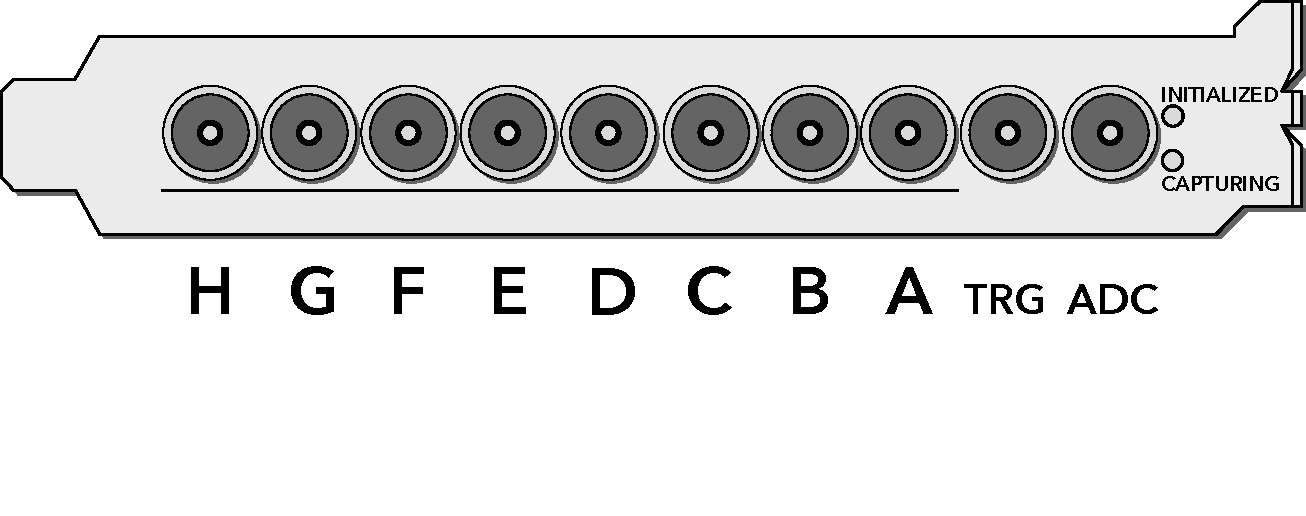
\includegraphics[width=0.6\textwidth]{%
                    figures/xHPTDC8_Slotblende.pdf}
            }{
                \includegraphics[width=0.6\textwidth]{%
                    figures/xTDC4_Slotblende.pdf}
            }
            \caption{
                Input connectors of the \deviceName\ on the PCIe
                bracket.%
                \ifxHPTDC{
                    Note, the TRG connector acts as a trigger only for the
                    ADC channel, not the TDC channels (see Section~\ref{adc}).
                }{}
                \label{fig:bracket}
            }
        \end{center}
    \end{figure*}
    %
    \begin{figure*}[hb]
        \begin{center}
            \ifxHPTDC{
                \includegraphics[width=0.3\textwidth]{%
                    xhptdc/figures/InputCircuit.pdf}
            }{
                \includegraphics[width=0.3\textwidth]{%
                    figures/InputCircuit.pdf}
            }
            \caption{
                Input circuit for each of the input
                channels.
                \ifxHPTDC{
                    Note, the TRG connector acts as a trigger only for the
                    ADC channel, not the TDC channels (see Section~\ref{adc}).
                }{}
                \label{fig:inputcirc}
            }
        \end{center}
    \end{figure*}
    %

    LEMO-00 connectors are used for input connection. The inputs are AC-coupled
    and have an impedance of 50\,Ω.  A schematic of the input circuit is shown
    in Figure \ref{fig:inputcirc}.  The digital threshold for any input can be
    adjusted to comply with a multitude of single-ended signaling standards. 
    The threshold can also be used to configure the input for either positive
    or negative pulses.
    
    The connectors can also be used as outputs. 
    \ifxHPTDC{AC-coupled}{DC-coupled} output pulses for automatic internal
    triggering and control of external devices can be generated using the
    TiGer timing pattern generator. See Section~\ref{cp:tiger} for details on
    the TiGer. 
    %
        \begin{figure*}[ht]
            \begin{center}
                \ifxHPTDC{
                    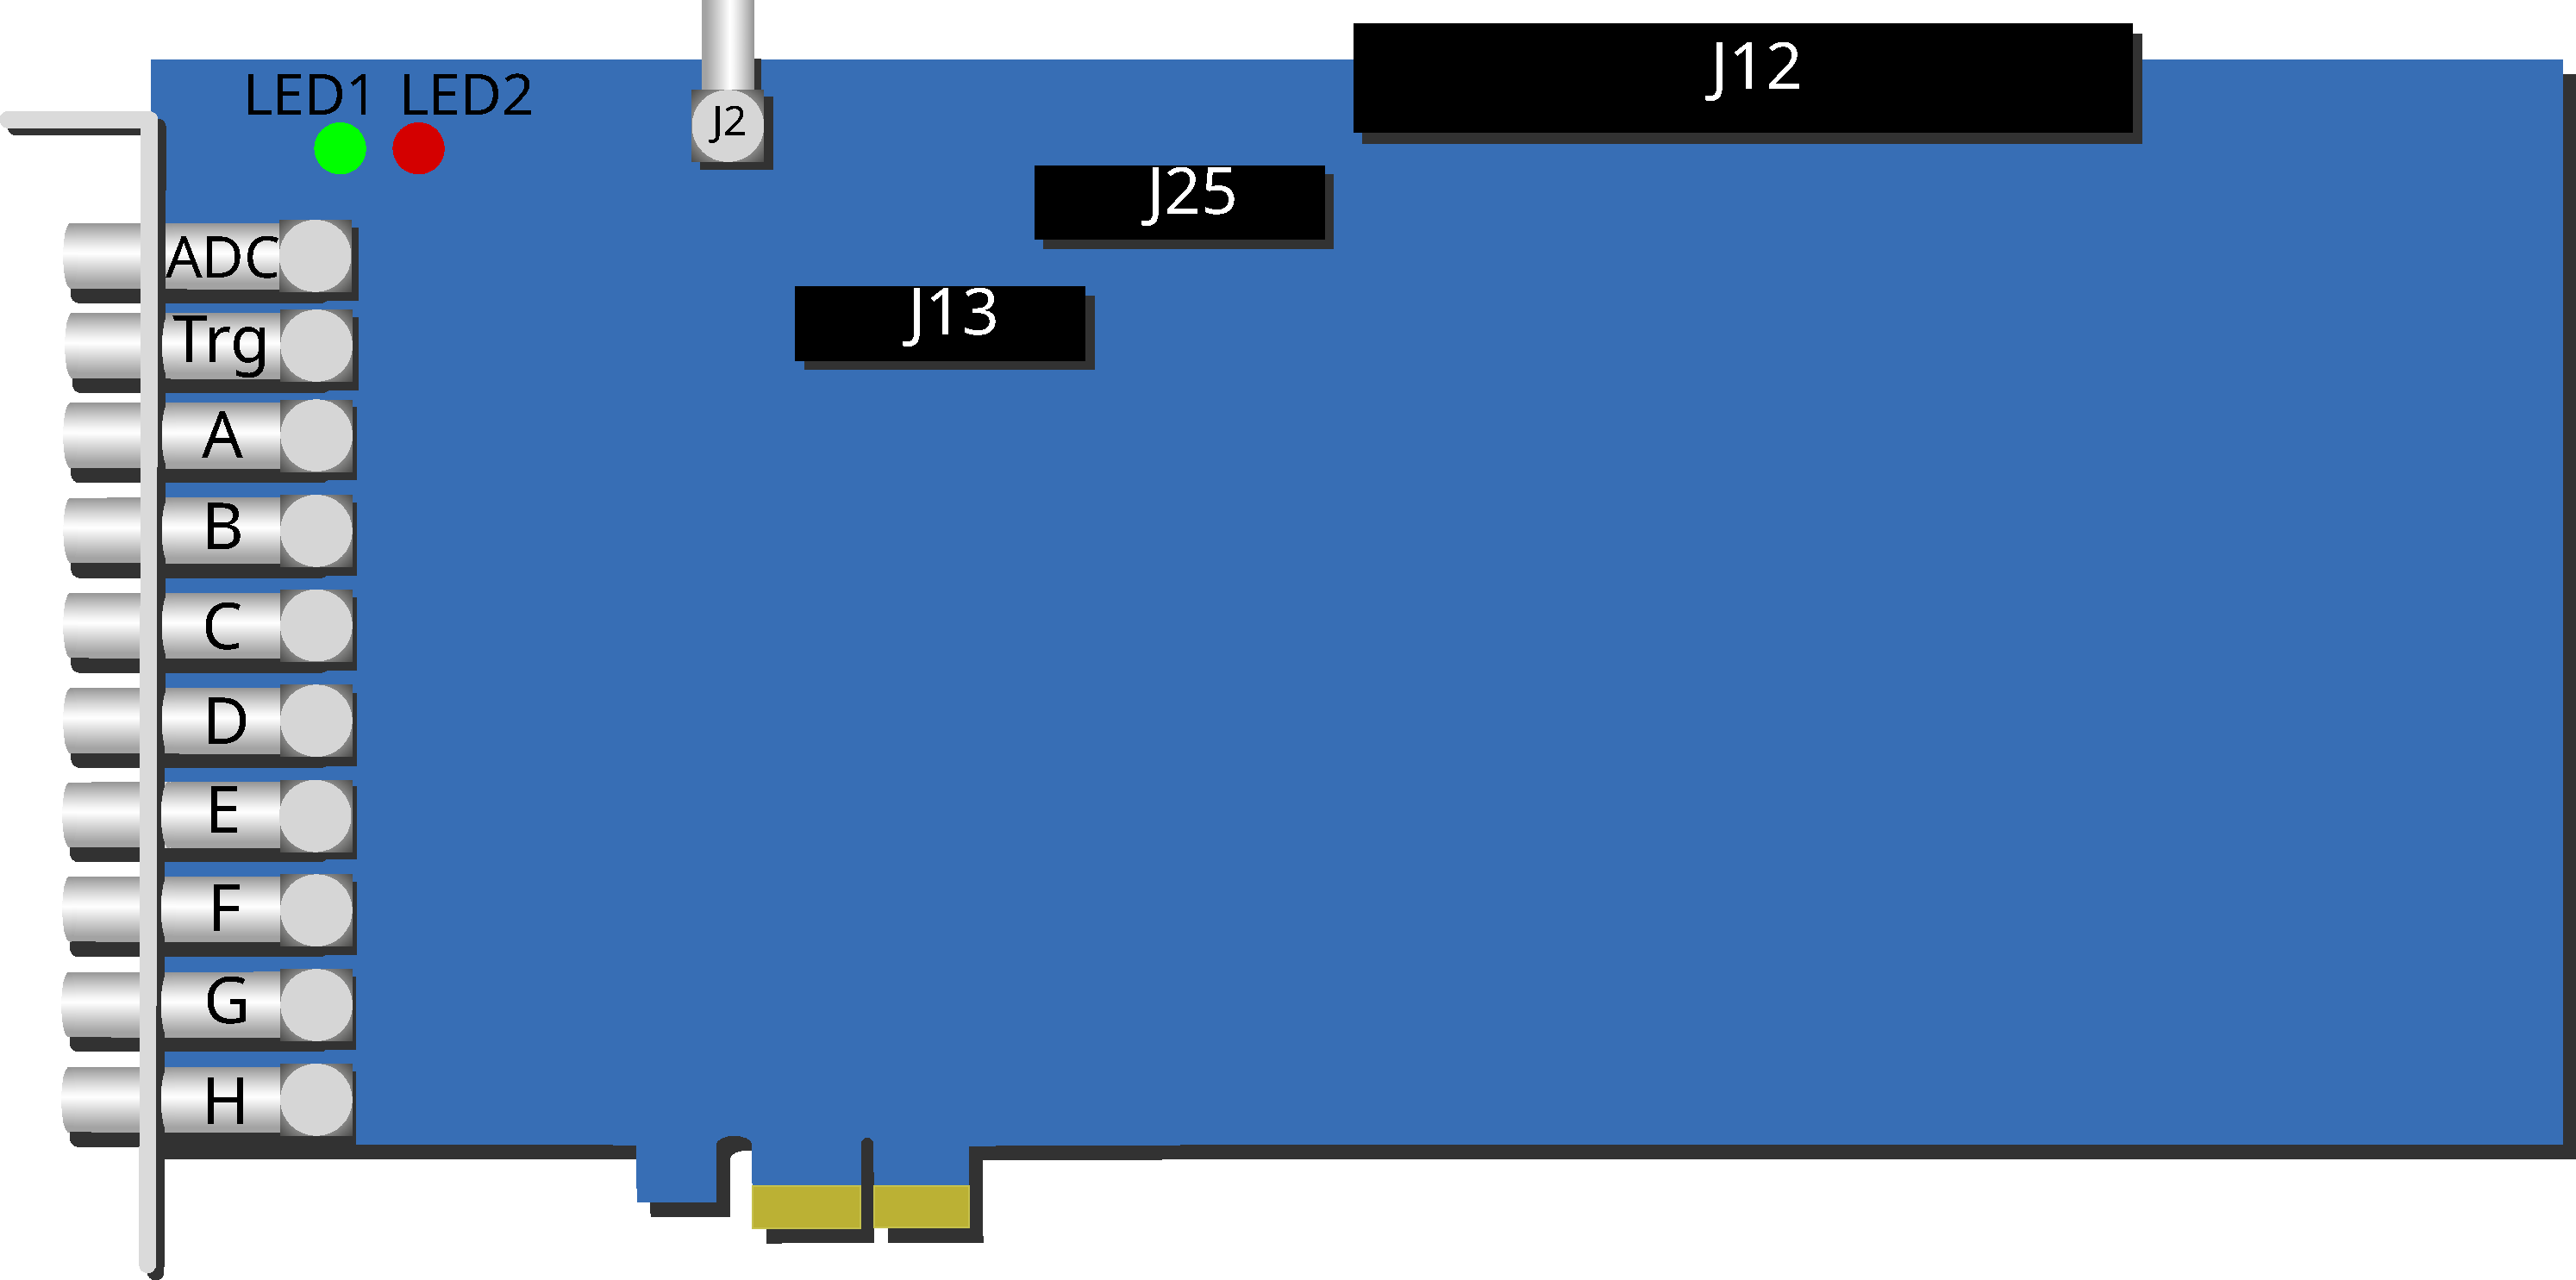
\includegraphics[width=0.7\textwidth]{%
                        xhptdc/figures/xHPTDC8_schematic.pdf}
                }{
                    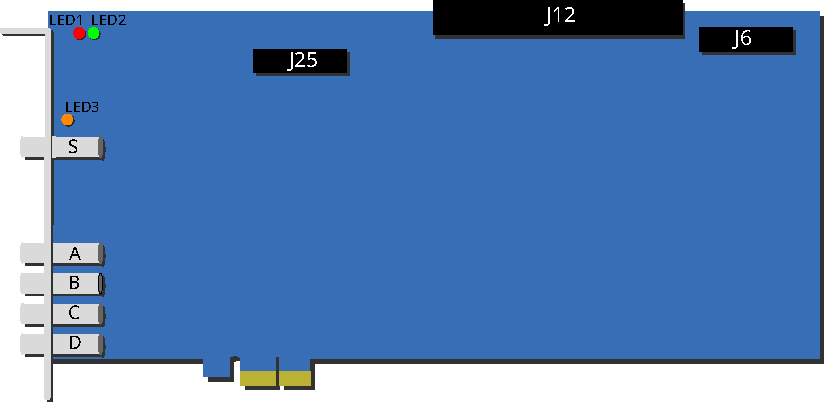
\includegraphics[width=0.7\textwidth]{%
                        figures/xTDC4_schematic.pdf}
                }
                \caption{Schematic view of \adeviceName\ Gen\,1 board showing
                    the inter-board connectors.\label{fig:schematics}}
            \end{center} 
        \end{figure*}
    %
    \ifxHPTDC{
        Furthermore three inter-board connectors can be found near the top
        edge of the \deviceName\ board, as displayed in
        Figure~\ref{fig:schematics}.  Connector J25 is reserved for future
        use. The pinout of connector J12 is shown in Table \ref{J12} and the
        pinout of connector J6 is depicted in Table~\ref{J6}.
        Connector J2 is a coax clock input that must receive a 10~MHz clock if
        multiple boards are used together as described in
        Section~\ref{multiboard}.
    }{%TT4 & xTDC4
        Furthermore, for Gen\,1 boards three inter-board connectors can be
        found near the top edge of the \deviceName\ board, as displayed in
        Figure~\ref{fig:schematics}.  Connector J25 is reserved for future
        use. The pinout of connector J12 is shown in Table \ref{J12} and the
        pinout of connector J6 is depicted in Table \ref{J6}. \textbf{Gen\,2
        boards do not posses these three connectors}.
    }

    \begin{table}
    \begin{small}
        \begin{center}
            \begin{tabular}{|c|c|}
                \hline
                Pin & Name\\
                \hline\hline
                1, 2 & GND\\
                \hline
                3, 4 & external CLK in N, external CLK in P\\
                \hline
                5, 6 & GND\\
                \hline
                7, 8 & reserved/NC\\
                \hline
                9, 10 & GND\\
                \hline
                11, 12 & reserved/NC\\
                \hline
                13, 14 & GND\\
                \hline
                15, 16 & reserved/NC\\
                \hline
                17, 18 & GND\\
                \hline
                19, 20 & reserved/NC\\
                \hline
                21, 22 & GND\\
                \hline
                23, 24 & reserved/NC\\
                \hline
                25, 26 & GND\\
                \hline
                27, 28 & reserved/NC\\
                \hline
                29, 30 & GND\\
                \hline
                31, 32 & reserved/NC\\
                \hline
                33, 34 & GND\\
                \hline
            \end{tabular}
            \caption{Pinout of connector J12.}
            \label{J12}
        \end{center}
    \end{small}
    \end{table}

    \begin{table}
    \begin{small}
        \begin{center}
            \begin{tabular}{|c|c|}
                \hline
                Pin & Name\\
                \hline\hline
                1 & +\SI{3.3}{\volt}\\
                \hline
                2 - 9 & reserved/NC\\
                \hline
                10 & GND\\
                \hline
            \end{tabular}
            \caption{Pinout of connector J6.}
            \label{J6}
        \end{center}
    \end{small}
    \end{table}

%%%%%%%%%%%%%%% LEDs
\section{Status LEDs}
Three status LEDs are present on the board, as seen in 
Figure~\ref{fig:schematics}.
\begin{itemize}
    \item LED1 lights up red during the configuration of the FPGA
        and turns off afterward. If it stays permanently lit, the
        configuration failed.
    \item LED2 lights up green after the board is initialized by the
        driver and turns off when the device is closed by the
        software.
    \item LED3 lights up green when capture is started, yellow after
        the first start signal was detected and red when groups are
        missing.
\end{itemize}

%%%%%%%%%%%%%%% multiboard
\ifxHPTDC{
    \section{Synchronizing multiple boards}
        \label{multiboard}
        If more than eight TDC inputs are required, up to six boards can be
        synchronized within a system. 
        
        The \deviceName\ API described in Chapter~\ref{cp:api} manages up to
        six boards automatically and provides a single data stream that
        contains sorted hit data from all boards in chronological order. 
        Channel A of each board is assigned channel number $\texttt{board\tu
        index} \times 10$.  The \texttt{board\tu index} is assigned to the
        boards in the order of the serial numbers starting at 0.

        \subsection{Connecting multiple boards}
            The boards must each receive a common \SI{10}{\mega\hertz} clock
            on connector J2. The connector is inside the PC enclosure. 
            Connectors J12 of all boards must be connected with a flat band
            cable with a terminator at each end.  Cable and Terminator are
            available from cronologic. See Figure~\ref{fig:multiboard} for a
            wiring example.  %
            \begin{figure*}[ht]
                \begin{center}
                    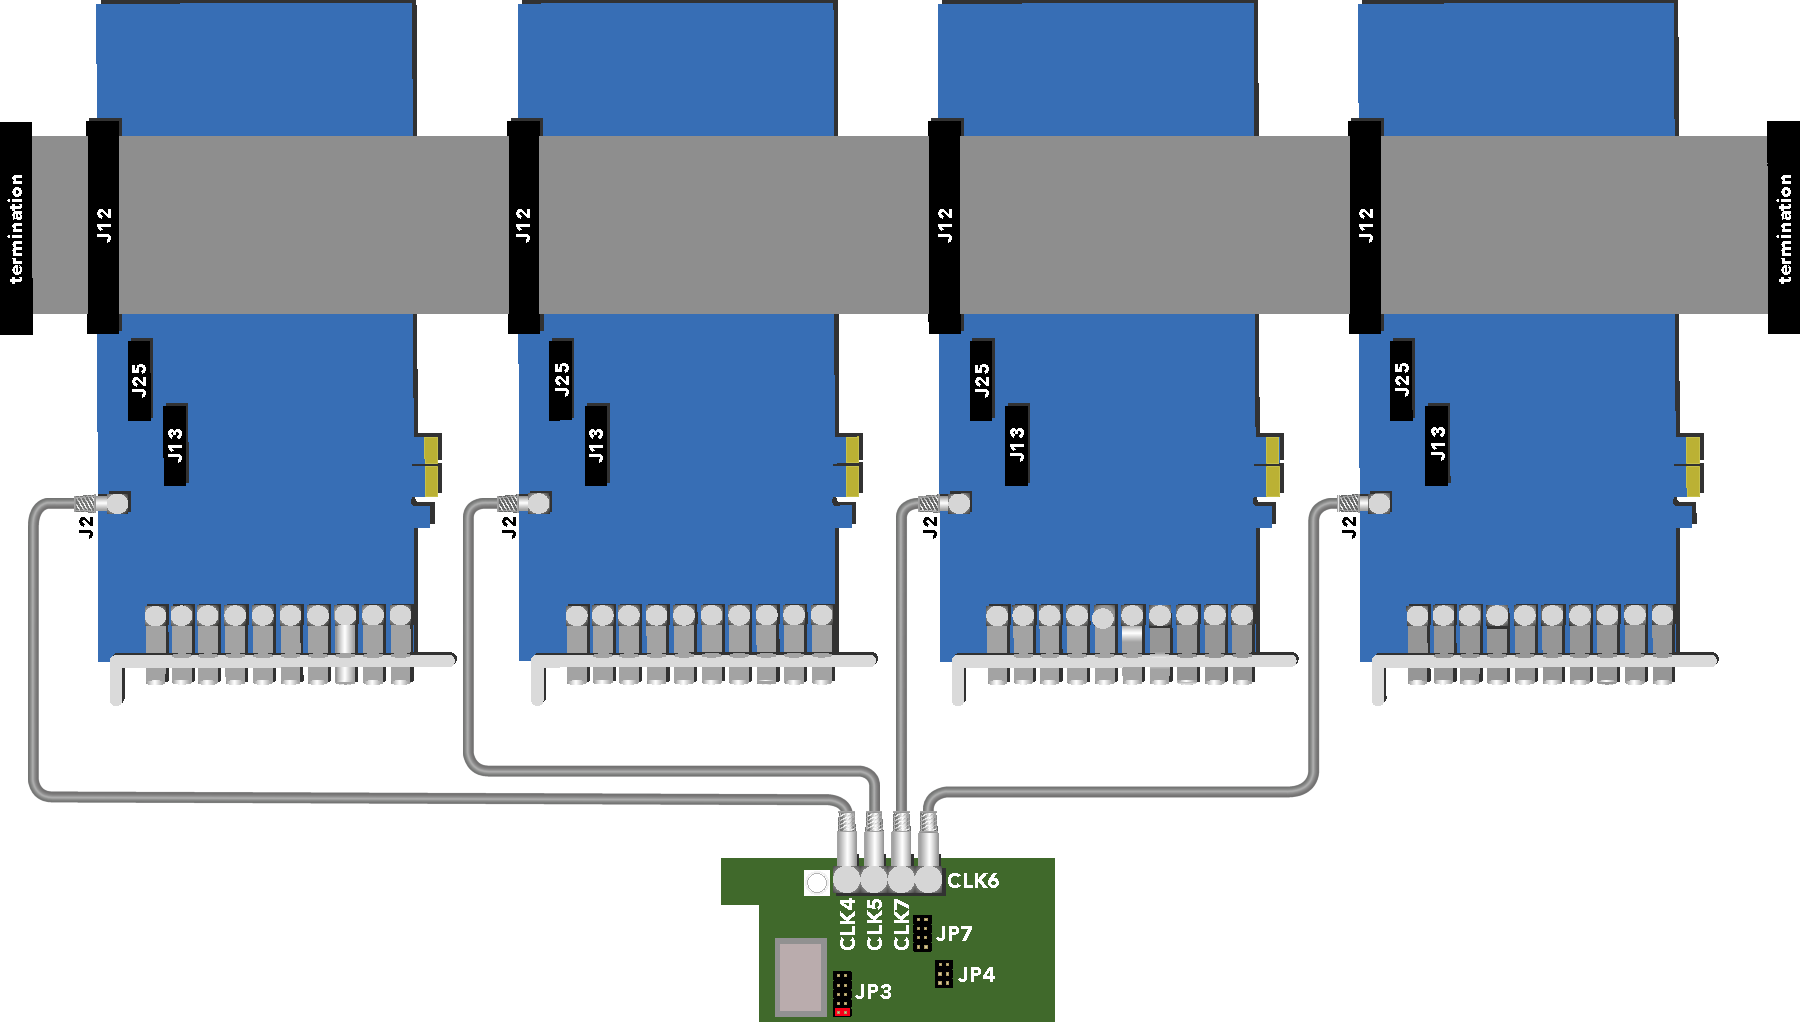
\includegraphics[width=1\textwidth]{
                        xhptdc/figures/multiboard.pdf}				
                    \caption{Synchronizing multiple boards with a
                        ClockBox.\label{fig:multiboard}}
                \end{center} 
            \end{figure*}
            %
        \subsection{ClockBox}
            For systems of up to four boards, cronologic offers the ClockBox
            product that conveniently makes four clock signals available
            inside the PC enclosure. For use with the \deviceName, jumper JP3
            of the ClockBox must be set as shown in Figure~\ref{fig:clockbox}
            in order to set the clock frequency to \SI{10}{\mega\hertz}. 
            %
            \begin{figure*}[ht]
                \begin{center}
                    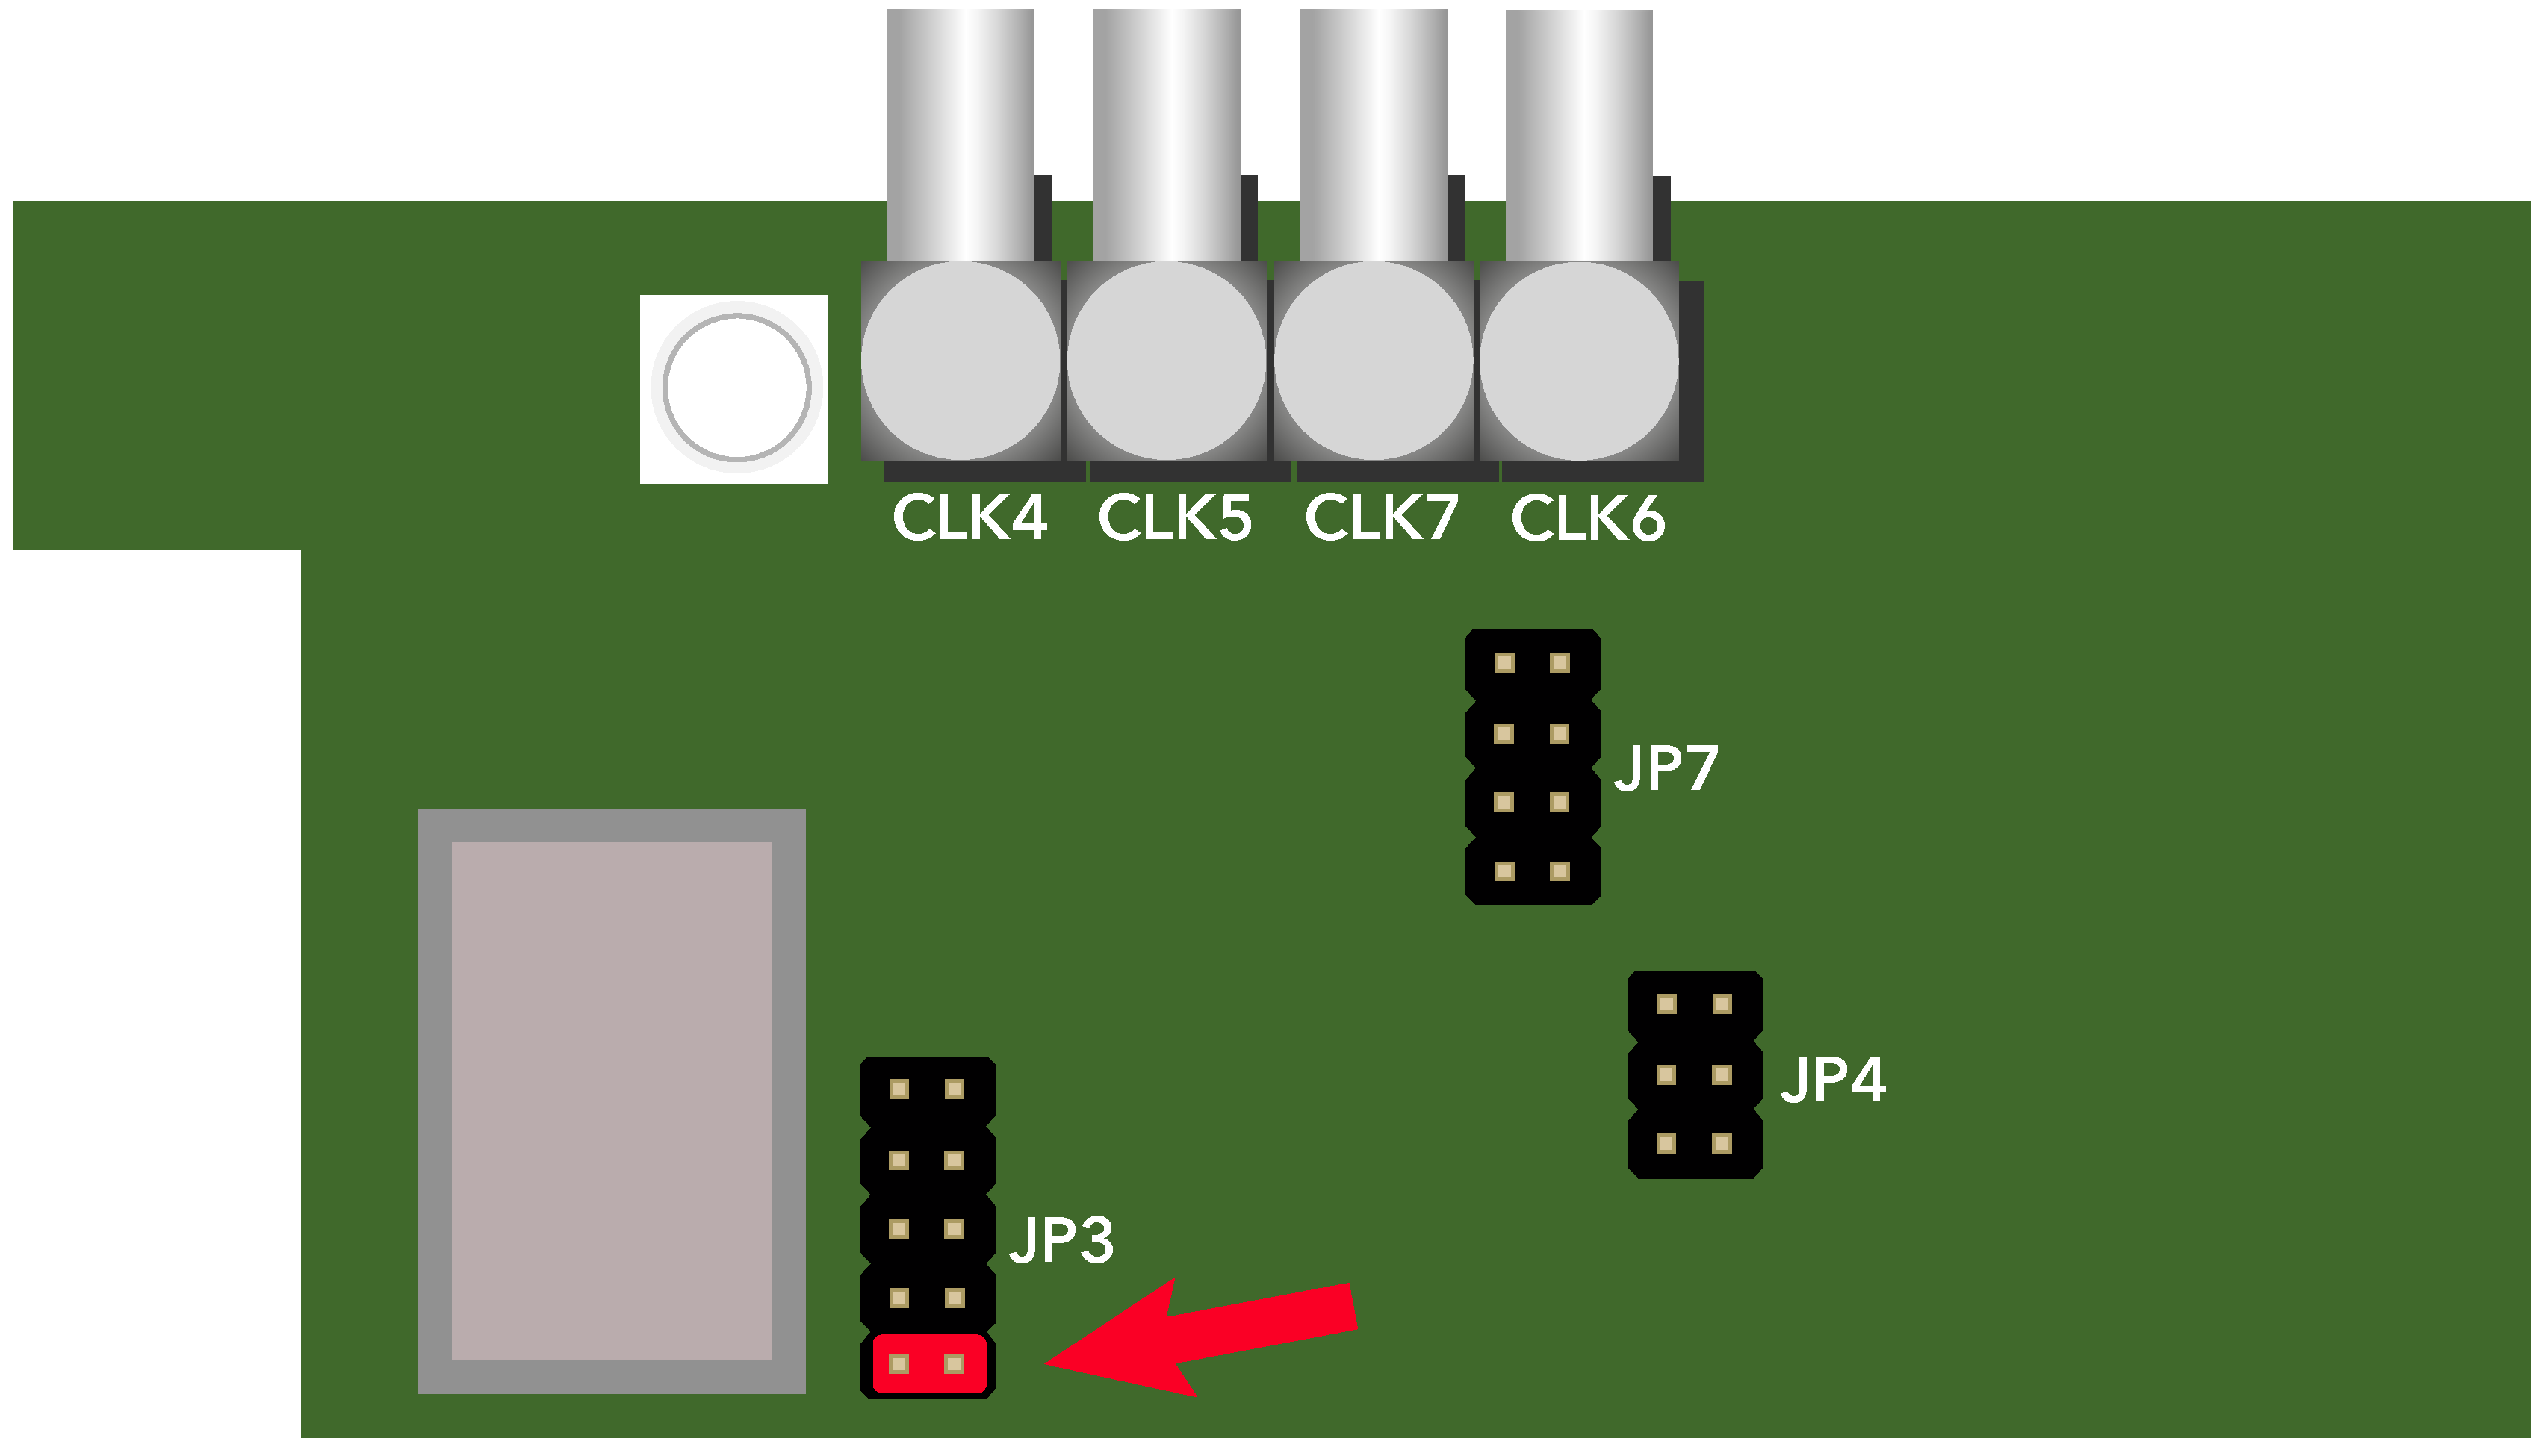
\includegraphics[width=0.5\textwidth]{
                        xhptdc/figures/clockbox.pdf}				
                    \caption{ClockBox jumper setting for
                        \SI{10}{\mega\hertz}.\label{fig:clockbox}}
                \end{center} 
            \end{figure*}
            %
        
        \subsection{Crates for multiple boards}
            Most PC mainboards don't have enough PCIe slots to support six
            \deviceName s.  We offer an external enclosure called ``Ndigo
            Crate'' that uses PCIe-over-cable technology to extend the number
            of available slots in a system.  The extension is fully
            transparent to the host system. There are no additional drivers
            required.  Please see the
            \href{https://www.cronologic.de/products/pcie/pcie-crates}{%
                product page} at our website \url{www.cronologic.de}.
}{}




    


